\documentclass{article}
\usepackage[utf8]{inputenc}
\usepackage{listings}
\usepackage{CJKutf8}
\usepackage{amsmath}
\usepackage{graphicx}
\usepackage[export]{adjustbox}
\title{Lab3 Report}
\author{b09901142 EE3 呂睿超}
\date{October 2022}

\usepackage{xcolor}

\definecolor{codegreen}{rgb}{0,0.6,0}
\definecolor{codegray}{rgb}{0.5,0.5,0.5}
\definecolor{codepurple}{rgb}{0.58,0,0.82}
\definecolor{backcolour}{rgb}{0.8,0.9,0.8}

\lstdefinestyle{mystyle}{
    backgroundcolor=\color{backcolour},   
    commentstyle=\color{codegreen},
    keywordstyle=\color{magenta},
    numberstyle=\tiny\color{codegray},
    stringstyle=\color{codepurple},
    basicstyle=\ttfamily\footnotesize,
    breakatwhitespace=false,         
    breaklines=true,                 
    captionpos=b,                    
    keepspaces=true,                 
    numbers=left,                    
    numbersep=5pt,                  
    showspaces=false,                
    showstringspaces=false,
    showtabs=false,                  
    tabsize=2
}

\lstset{style=mystyle}





\begin{document}
\begin{CJK*}{UTF8}{bsmi}
\maketitle

\section{The Deutsch–Jozsa algorithm}
\subsection{(a)}
\begin{enumerate}
\item In order to complete a truth table, I generated a list with all the binary values that was derived from decimal vales.
\item I followed the instructions and finished the oracle circuits.The Python implementation of the balanced function oracle is in \emph {Appendix 1}:

\item Then I use the 'qasm simulator' to observe the result, which fits my expectation.
The output of the first oracle are all zeros. The output of the second oracle are all ones.
The output of the last oracle are equal zeros and ones which is verified by truth-table.count('0') = truth-table.count('1').

\end{enumerate}
\subsection{(b)} 
\begin{enumerate}
\item I followed the instruction in the Qiskit Textbook, and generalized the circuit. The circuit implementation is as the lecture note shows. First, create a superposition state of the first n qubits. Add an ancilla bit in minus state. Append the oracle circuit. Apply n Hadamard gates and discard the ancilla. Measure the first n qubits.

\item Using the plot-histogram function, the results verified the theorem. When testing oracle is constant, the output is zero outcomes certainly.({'0000':1024})
When testing oracle is balanced, the output is non-zero outcomes certainly.As the simulator is ideal, the outcome is a all one bit string({'1111':1024})
\end{enumerate}


\section{Grover's Search}
\subsection{(a)} 
\begin{enumerate}
    \item Following the instructions, I implemented the phase flip oracle. Notice that in the statevector representation, x = '011' is in the seventh component.  

    \item For testing, I prepared a superposition state with each coefficient = $\frac{1}{\sqrt{8}}$ i.e.  $statevector = \begin{bmatrix}
    \frac{1}{\sqrt{8}} \frac{1}{\sqrt{8}} \frac{1}{\sqrt{8}} \frac{1}{\sqrt{8}} \frac{1}{\sqrt{8}} \frac{1}{\sqrt{8}} \frac{1}{\sqrt{8}} \frac{1}{\sqrt{8}}
    \end{bmatrix}$
    
    \item After the oracle, the  $statevector = \begin{bmatrix}
    \frac{1}{\sqrt{8}} \frac{1}{\sqrt{8}} \frac{1}{\sqrt{8}} \frac{1}{\sqrt{8}} \frac{1}{\sqrt{8}} \frac{1}{\sqrt{8}} \frac{-1}{\sqrt{8}} \frac{1}{\sqrt{8}}
    \end{bmatrix}$
    
\end{enumerate}

\subsection{(b)}
Following, the lecture note,I implemented the inverse about mean circuit as below.
    \begin{figure}[h]
    \centering
    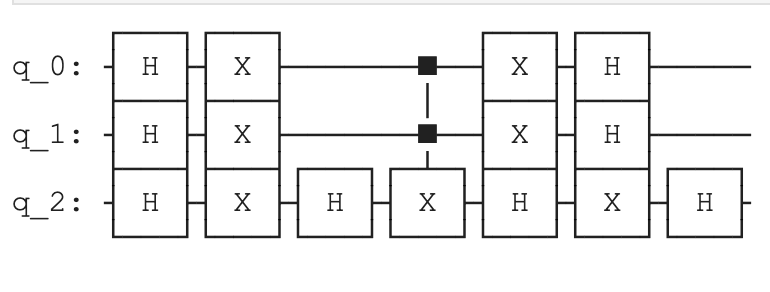
\includegraphics[width=0.9\textwidth]{2b.png}
    \caption{\label{fig:2b.png}2(b) Inverse about mean.}
    \end{figure}

The circuit first apply Hadamard gates, then not gates, then a multi-control z gate implemented by toffoli gate and h gates, then not gate, finally h gates.

The implementing code are in \emph {Appendix 5}

\subsection{(c)}
Next, I generalize the grover's algorithm into a function. The circuit figure is shown below. The first sub-circuit is the phase flip oracle, while the second is the inverse about mean circuit.
\begin{figure}[h]
    \centering
    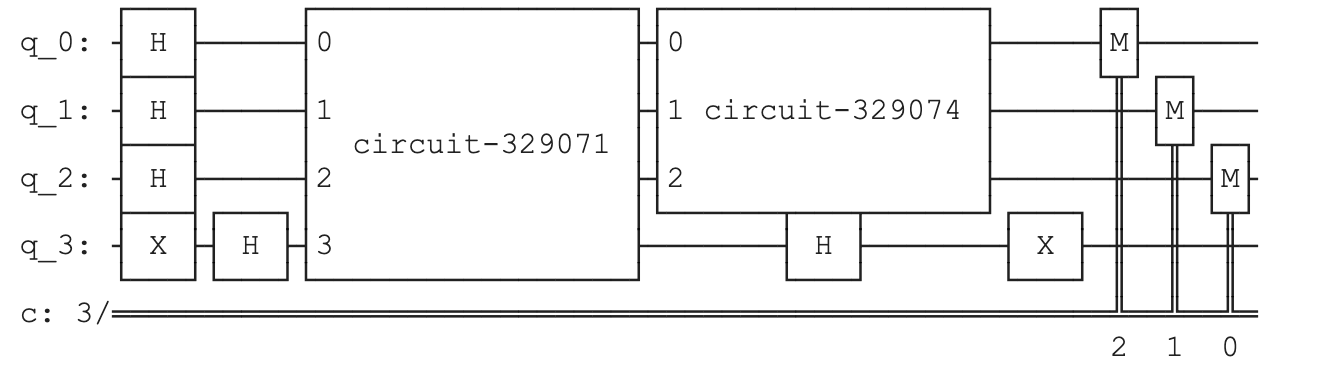
\includegraphics[width=0.9\textwidth]{2c.png}
    \caption{\label{fig:2c.png}2(c) DJ circuit.}
    \end{figure}

After testing, my simulating circuit can find x = '011' over 50 percent probabilities in most iterations. An interesting fact is that in some iteration, the probability of measuring x = '011' is lowest.
Below presents two figures of the result from iteration 1 and iteraion 9
\begin{enumerate}
    \item result of iteration 1
    \begin{figure}[h]
    \centering
    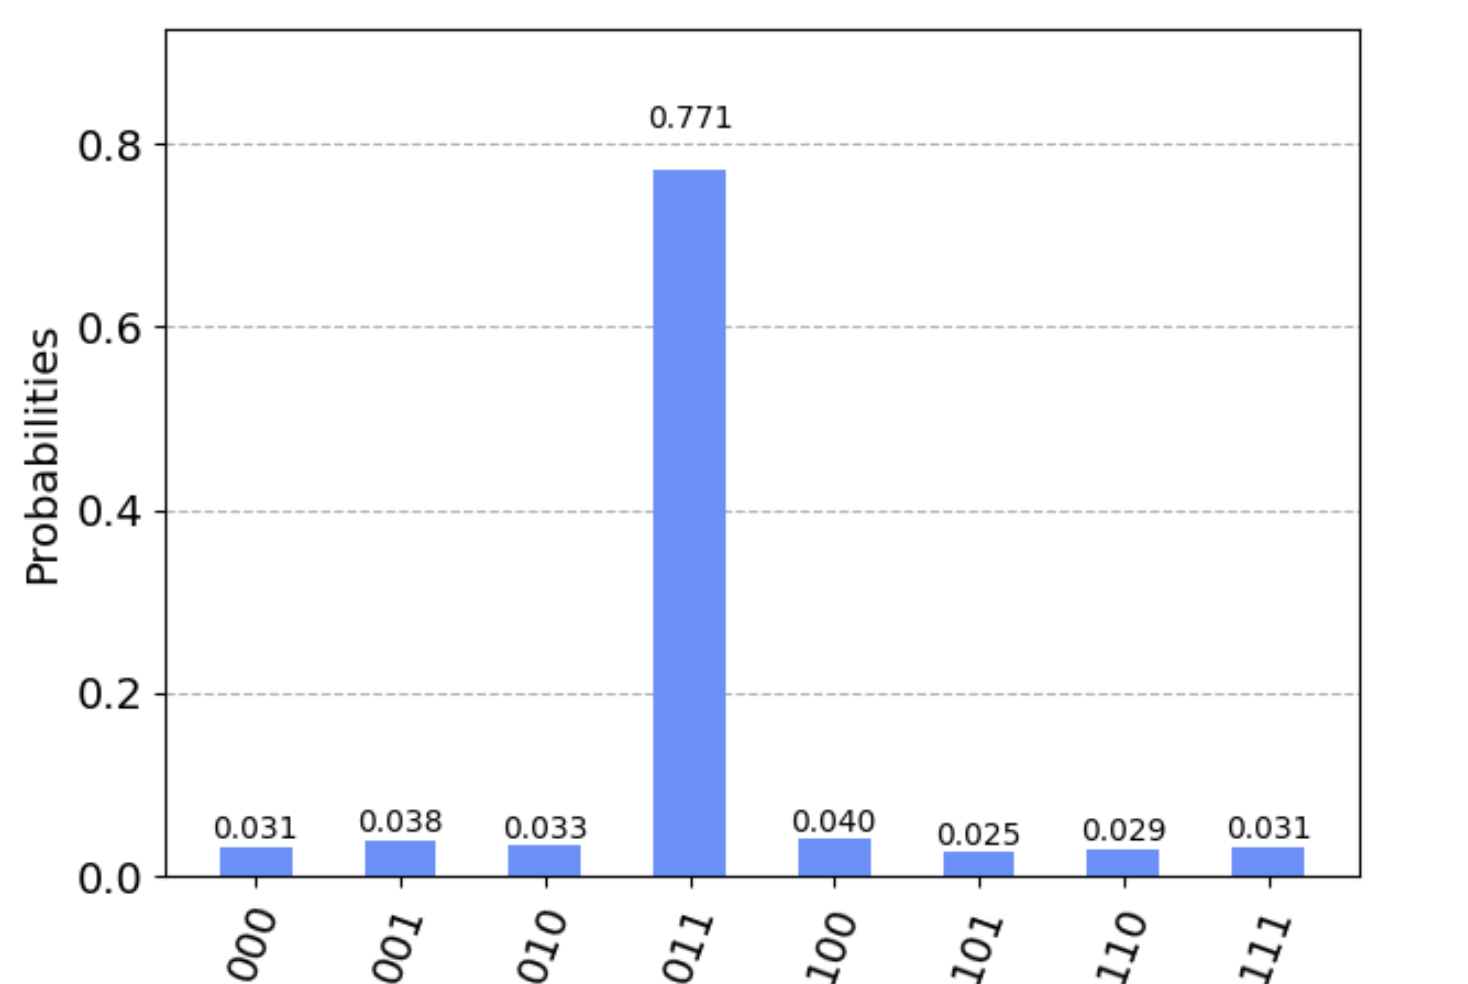
\includegraphics[width=0.7\textwidth]{1.png}
    \caption{\label{fig:1.png}2(c)}
    \end{figure}
    \item result of iteration 9
    \begin{figure}[h]
    \centering
    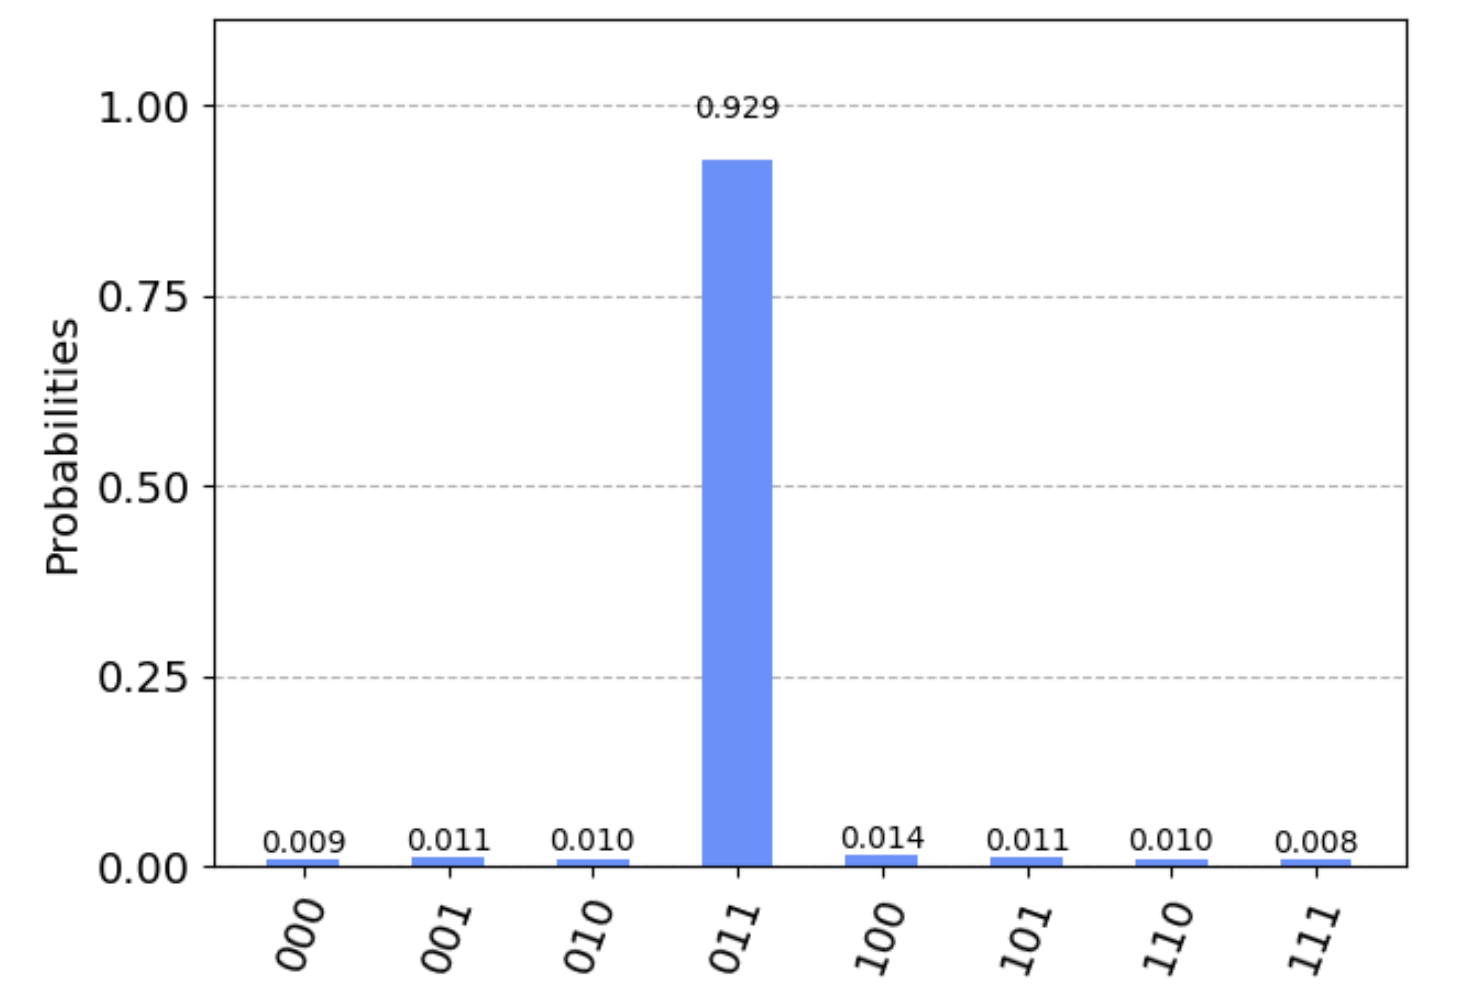
\includegraphics[width=0.7\textwidth]{9.png}
    \caption{\label{fig:9.png}2(c)}
    \end{figure}
\end{enumerate}
\subsection{(d)}
\begin{enumerate}
    \item Following the instructions, I implemented the new phase flip oracle.  

    \item For testing, I prepared a superposition state with each coefficient = $\frac{1}{\sqrt{8}}$ i.e. $statevector = \begin{bmatrix}
    \frac{1}{\sqrt{8}} \frac{1}{\sqrt{8}} \frac{1}{\sqrt{8}} \frac{1}{\sqrt{8}} \frac{1}{\sqrt{8}} \frac{1}{\sqrt{8}} \frac{1}{\sqrt{8}} \frac{1}{\sqrt{8}}
    \end{bmatrix}$
    
    \item After the oracle, the  $statevector = \begin{bmatrix}
    \frac{1}{\sqrt{8}} \frac{1}{\sqrt{8}} \frac{1}{\sqrt{8}} \frac{1}{\sqrt{8}} \frac{1}{\sqrt{8}} \frac{-1}{\sqrt{8}} \frac{-1}{\sqrt{8}} \frac{1}{\sqrt{8}}
    \end{bmatrix}$
    which fits the expectation.
\end{enumerate}

\subsection{(e)}
After the search algorithm, I get the simulation result $Prob('011') \approx Prob('101') \approx 0.5$

\subsection{(f)}

\section{Quantum Fourier Transform}
For this section, I only followed the instructions and implemented the code.
\section{Period-Finding Algorithm}
For this section, I only followed the instructions and implemented the code.
\section{Appendix}
\subsection{balanced function oracle implementation}
\begin{lstlisting}[language=Python]
n = 4
#generate all binary inputs
all_pos = []
for i in range(2**n):
    temp = i
    temp = bin(temp)
    temp = temp[2:]
    while(len(temp)<n):
        temp = '0' + temp
    all_pos.append(temp)
truth_table = []
for pos in all_pos:
    circuit3 = QuantumCircuit(5,1)
    for j in range(len(pos)):
        if pos[j] == '1':
            circuit3.x(j)
    for i in range(n):
        circuit3.cnot(i,4)
    circuit3.measure(4,0)
    simulator = Aer.get_backend('qasm_simulator')
    job = execute(circuit3, simulator, shots = 1024)
    result = job.result()
    counts = result.get_counts()
    for key, value in counts.items():
        res = key
    truth_table.append(res)
print(truth_table)
print(truth_table.count('0'))
print(truth_table.count('1'))
\end{lstlisting}



\end{CJK*}
\end{document}
